% Shor's algorithm as quantum circuits -- factoring and ECDLP in Qiskit.
% Theme and layout follow doc/references/shor_pres_v4_1.pdf.
%
%   ../venv/bin/python make_figures.py     # figures/ and numbers.json, computed from shor_qiskit/
%   ../venv/bin/python make_listings.py    # listings/, cut from the source and checked
%   tectonic -X compile shor_circuits.tex
\documentclass[aspectratio=169,11pt]{beamer}

% --- fonts: Palatino throughout, as in shor_pres_v4_1 --------------------------
\usepackage{mathpazo}
\usepackage{fontspec}
\setmainfont{texgyrepagella}[Extension=.otf,UprightFont=*-regular,BoldFont=*-bold,ItalicFont=*-italic,BoldItalicFont=*-bolditalic]
\setsansfont{texgyrepagella}[Extension=.otf,UprightFont=*-regular,BoldFont=*-bold,ItalicFont=*-italic,BoldItalicFont=*-bolditalic]
\setmonofont{Inconsolatazi4}[Extension=.otf,UprightFont=*-Regular,BoldFont=*-Bold,Scale=0.92]
\usefonttheme{serif}

\usepackage{amsmath,amssymb,booktabs,graphicx,listings,appendixnumberbeamer}
\usepackage[most]{tcolorbox}
\usepackage{tikz}
\usetikzlibrary{arrows.meta,positioning,calc,fit,decorations.pathreplacing}

% --- colours, sampled from shor_pres_v4_1 --------------------------------------
\definecolor{ink}{HTML}{1A1C20}
\definecolor{body}{HTML}{3A4550}
\definecolor{subtle}{HTML}{6E747E}
\definecolor{rulegrey}{HTML}{C7C4BE}
\definecolor{quotebar}{HTML}{757D84}
\definecolor{cblue}{HTML}{1A5FA0}      % the counting register
\definecolor{cverm}{HTML}{B3401A}      % the target register, arithmetic
\definecolor{cpurple}{HTML}{63389B}    % the period, the key, angles
\definecolor{indigo}{HTML}{52439A}
\definecolor{lavender}{HTML}{F5F4F9}
\definecolor{greybox}{HTML}{F4F3F0}
\definecolor{peach}{HTML}{FAF2ED}
\newcommand{\cnt}[1]{\textcolor{cblue}{#1}}
\newcommand{\tgt}[1]{\textcolor{cverm}{#1}}
\newcommand{\per}[1]{\textcolor{cpurple}{#1}}

% --- frame furniture -------------------------------------------------------------
\setbeamertemplate{navigation symbols}{}
\setbeamercolor{normal text}{fg=ink}
\setbeamercolor{structure}{fg=ink}
\setbeamerfont{frametitle}{series=\bfseries,size=\large}
\setbeamertemplate{frametitle}{%
  \vskip2.2mm\usebeamerfont{frametitle}\insertframetitle\par\vskip1.4mm
  {\color{rulegrey}\rule{\textwidth}{0.4pt}}\vskip-0.5mm}
\setbeamertemplate{footline}{%
  \hfill{\scriptsize\color{ink}\insertframenumber\,/\,\inserttotalframenumber}\hspace*{5mm}\vskip3mm}
\setbeamertemplate{itemize item}{\small\raise0.3ex\hbox{\textbullet}}
\setbeamertemplate{enumerate item}{\insertenumlabel.}
\setbeamersize{text margin left=7mm,text margin right=7mm}
\setlength{\parskip}{3pt}

% --- boxes -----------------------------------------------------------------------
\tcbset{base/.style={enhanced,sharp corners,boxrule=0pt,frame hidden,left=5pt,right=5pt,
                     top=3pt,bottom=3pt,before skip=5pt,after skip=5pt}}
\newtcolorbox{difficulty}[1]{base,colback=lavender,borderline west={2pt}{0pt}{indigo},
  before upper={\textbf{\color{indigo}Difficulty #1.}\ }}
\newtcolorbox{greyblock}[1][]{base,colback=greybox,#1}
\newtcolorbox{peachblock}[1][]{base,colback=peach,#1}
\newtcolorbox{takeaway}[1][]{base,colback=white,borderline west={2pt}{0pt}{quotebar},
  fontupper=\itshape,left=7pt,#1}
\newcommand{\blocktitle}[1]{{\bfseries #1}\par\smallskip}
\newcommand{\peachtitle}[1]{{\bfseries\color{cverm}#1}\par\smallskip}
\newcommand{\resolved}[1]{\begin{takeaway}\textbf{Resolved.} #1\end{takeaway}}

% --- code ---------------------------------------------------------------------------
\lstdefinestyle{py}{language=Python,basicstyle=\ttfamily\footnotesize,
  keywordstyle=\color{indigo}\bfseries,commentstyle=\color{subtle}\itshape,
  stringstyle=\color{cverm},showstringspaces=false,columns=fullflexible,keepspaces=true,
  backgroundcolor=\color{greybox},frame=none,xleftmargin=5pt,framexleftmargin=5pt,
  framextopmargin=3pt,framexbottommargin=3pt,aboveskip=3pt,belowskip=3pt,upquote=true,
  morekeywords={with,as,assert}}
\lstset{style=py}
\newcommand{\code}[2][]{\lstinputlisting[#1]{listings/#2}}

% --- act dividers, as in shor_pres_v4_1: centred, unnumbered ---------------------------
\newcommand{\act}[1]{{\setbeamertemplate{footline}{}%
  \begin{frame}[noframenumbering]\vfill\centering{\Large #1\par}\vfill\end{frame}}}
\newcommand{\fig}[2][]{\includegraphics[#1]{figures/#2}}

% --- circuit schematics -------------------------------------------------------------
\tikzset{
  wire/.style={thick,color=body},
  cwire/.style={thick,color=cblue},
  twire/.style={thick,color=cverm},
  clw/.style={color=quotebar,double,double distance=1.2pt},
  op/.style={draw=cverm,fill=cverm!8,thick,font=\small,inner sep=2pt,align=center},
  qop/.style={draw=cpurple,fill=cpurple!8,thick,font=\small,inner sep=2pt},
  hop/.style={draw=cblue,fill=white,thick,minimum size=5mm,font=\small,inner sep=1pt},
  dot/.style={circle,fill=body,inner sep=0pt,minimum size=1.8mm},
  meter/.style={draw=quotebar,fill=white,minimum size=5mm,font=\scriptsize,inner sep=1pt},
  lab/.style={font=\small,anchor=east},
  note/.style={font=\scriptsize,color=subtle,align=center},
}
\newcommand{\bundle}[3]{\draw[thick,color=body] (#1-0.07,#2-0.13) -- (#1+0.07,#2+0.13);
  \node[font=\tiny,color=subtle,above right=-1pt] at (#1,#2) {#3};}
\newcommand{\oplusat}[2]{\draw[thick,color=body] (#1,#2) circle (1.6mm);
  \draw[thick,color=body] (#1-0.16,#2) -- (#1+0.16,#2); \draw[thick,color=body] (#1,#2-0.16) -- (#1,#2+0.16);}

\begin{document}

% =====================================================================================
{\setbeamertemplate{footline}{}
\begin{frame}[noframenumbering]
  \vfill
  {\LARGE\bfseries Shor's Algorithm as Quantum Circuits\par}
  \vskip3mm
  {\itshape How factoring and the elliptic-curve discrete logarithm are built, run and costed\\
   --- from the textbook circuit to the optimised ones, in Qiskit\par}
  \vskip3mm{\color{rulegrey}\rule{0.62\textwidth}{0.4pt}}
  \vfill
\end{frame}}

\begin{frame}{How to read these slides}
  \begin{columns}[T]
    \begin{column}{0.47\textwidth}
      \blocktitle{Colours carry meaning}
      \cnt{Blue} --- the counting register, the one we measure.\par
      \tgt{Vermillion} --- the target register, where the arithmetic happens.\par
      \per{Purple} --- what we are after: the period $r$, the key $k$, the angles they produce.\par
      \vskip2mm
      {\color{subtle}\small Colour is a reminder, never the only carrier of information.}
    \end{column}
    \begin{column}{0.47\textwidth}
      \blocktitle{Each act is one question and its answer}
      \begin{difficulty}{}Opens each act: the obstacle to get past.\end{difficulty}
      \resolved{Closes the act: how it was removed.}
      \begin{peachblock}\peachtitle{Costs}qubits, Toffolis, T gates\end{peachblock}
      {\color{subtle}\small Every number is computed by the code in \texttt{shor\_qiskit/}, as in \texttt{notebooks/shor\_walkthrough.ipynb}.}
    \end{column}
  \end{columns}
\end{frame}

\begin{frame}{The road map, in plain words}
  \centering
  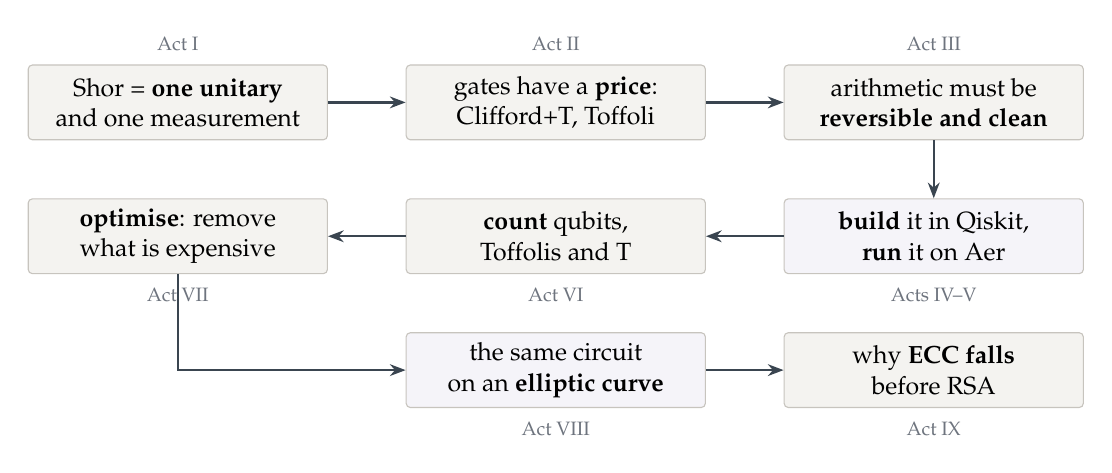
\begin{tikzpicture}[
      stage/.style={draw=rulegrey,fill=greybox,rounded corners=1.5pt,align=center,
                    minimum width=38mm,minimum height=9.5mm,font=\small},
      quantum/.style={stage,fill=lavender},
      lb/.style={font=\scriptsize,color=subtle},
      arr/.style={-{Stealth[length=2mm]},color=body,thick}]
    \node[stage]   (a) at (0,0)      {Shor = \textbf{one unitary}\\and one measurement};
    \node[stage]   (b) at (4.8,0)    {gates have a \textbf{price}:\\Clifford+T, Toffoli};
    \node[stage]   (c) at (9.6,0)    {arithmetic must be\\\textbf{reversible and clean}};
    \node[quantum] (d) at (9.6,-1.7) {\textbf{build} it in Qiskit,\\\textbf{run} it on Aer};
    \node[stage]   (e) at (4.8,-1.7) {\textbf{count} qubits,\\Toffolis and T};
    \node[stage]   (f) at (0,-1.7)   {\textbf{optimise}: remove\\what is expensive};
    \node[quantum] (g) at (4.8,-3.4) {the same circuit\\on an \textbf{elliptic curve}};
    \node[stage]   (h) at (9.6,-3.4) {why \textbf{ECC falls}\\before RSA};
    \foreach \u/\v in {a/b,b/c,c/d,d/e,e/f,g/h} \draw[arr] (\u) -- (\v);
    \draw[arr] (f.south) |- (g.west);
    \node[lb,above=0.5mm of a] {Act I};  \node[lb,above=0.5mm of b] {Act II};
    \node[lb,above=0.5mm of c] {Act III}; \node[lb,below=0.5mm of d] {Acts IV--V};
    \node[lb,below=0.5mm of e] {Act VI};  \node[lb,below=0.5mm of f] {Act VII};
    \node[lb,below=0.5mm of g] {Act VIII};\node[lb,below=0.5mm of h] {Act IX};
  \end{tikzpicture}
  \begin{takeaway}The quantum part of Shor is short. Almost all of its cost is reversible arithmetic --- that is what we build, run and count.\end{takeaway}
\end{frame}

% =====================================================================================
\act{Act I --- Shor's algorithm is one unitary and one measurement}

\begin{frame}{Act I --- factoring reduces to finding a period}
  \begin{difficulty}{1}To factor $N$, pick $a$ with $\gcd(a,N)=1$ and find its \textbf{order} \per{$r$}: the smallest $r>0$ with $a^r\equiv1 \pmod N$.\end{difficulty}
  \vskip1mm
  \centering
  \renewcommand{\arraystretch}{1.2}
  \begin{tabular}{c|ccccccc}
    $x$ & 0 & 1 & 2 & 3 & 4 & 5 & $\cdots$\\ \hline
    $7^x \bmod 15$ & 1 & 7 & 4 & 13 & 1 & 7 & $\cdots$
  \end{tabular}
  \qquad $\Rightarrow\ \per{r=4}$
  \vskip3mm
  \raggedright
  Why the period factors $N$: if $r$ is even, $N$ divides
  \[ a^r-1=(a^{r/2}-1)(a^{r/2}+1), \]
  and unless $a^{r/2}\equiv-1$ each factor shares a divisor with $N$: \ $\gcd(48,15)=3$, \ $\gcd(50,15)=5$.
  \begin{takeaway}The period is a property of the whole sequence, not of any one value. Only the period needs a quantum computer; the rest is Euclid.\end{takeaway}
\end{frame}

\begin{frame}{Phase estimation: the circuit}
  \centering
  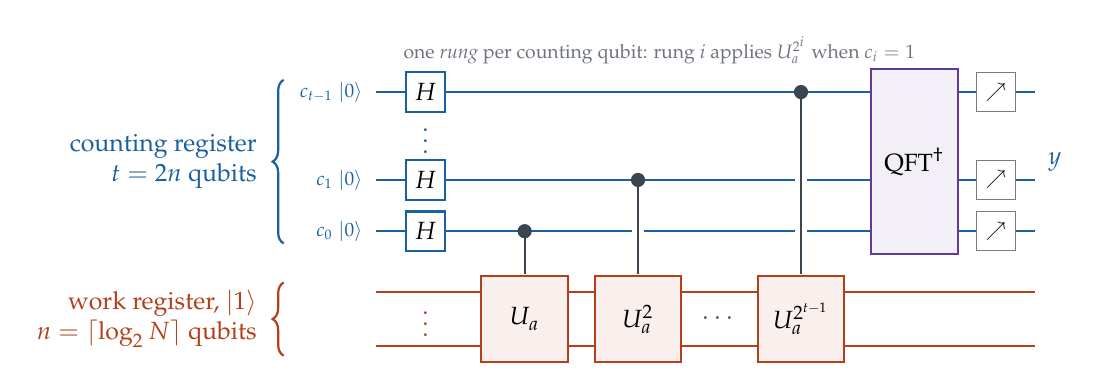
\begin{tikzpicture}[x=9mm,y=6.2mm]
    % counting register: c_0 at the bottom, c_{t-1} at the top; the gap row carries the dots
    \foreach \y/\q in {5.45/{t-1},3.65/1,2.6/0} {
      \node[font=\scriptsize,color=cblue,anchor=east] at (-0.05,\y) {$c_{\q}\;|0\rangle$};
      \draw[cwire] (0,\y) -- (9.3,\y);
      \node[hop] at (0.7,\y) {$H$};}
    \node[font=\small,color=cblue] at (0.7,4.62) {$\vdots$};
    % work register: n qubits holding the integer 1
    \foreach \y in {1.35,0.25} \draw[twire] (0,\y) -- (9.3,\y);
    \node[font=\small,color=cverm] at (0.7,0.86) {$\vdots$};
    % braces
    \draw[decorate,decoration={brace,amplitude=4pt},thick,color=cblue] (-1.3,2.35) -- (-1.3,5.7)
      node[midway,left=6pt,font=\small,align=right,color=cblue] {counting register\\$t=2n$ qubits};
    \draw[decorate,decoration={brace,amplitude=4pt},thick,color=cverm] (-1.3,0.05) -- (-1.3,1.55)
      node[midway,left=6pt,font=\small,align=right,color=cverm] {work register, $|1\rangle$\\$n=\lceil\log_2N\rceil$ qubits};
    % rungs: each control line hops over the wires it crosses
    \foreach \x/\y/\p in {2.1/2.6/{}, 3.7/3.65/{2}, 6.0/5.45/{2^{t-1}}} {
      \draw[white,line width=4pt] (\x,\y-0.28) -- (\x,1.75);
      \draw[thick,color=body] (\x,\y) -- (\x,1.72);
      \node[dot] at (\x,\y) {};
      \node[op,minimum width=11mm,minimum height=11mm] at (\x,0.8) {$U_a^{\p}$};}
    \node[font=\small,color=body] at (4.85,0.8) {$\cdots$};
    % inverse QFT and readout
    \node[qop,minimum height=23.5mm,minimum width=11mm] at (7.6,4.025) {$\mathrm{QFT}^\dagger$};
    \foreach \y in {5.45,3.65,2.6} \node[meter] at (8.75,\y) {$\nearrow$};
    \node[font=\small,color=cblue,anchor=west] at (9.35,4.025) {$y$};
    \node[note] at (4.0,6.3) {one \emph{rung} per counting qubit: rung $i$ applies $U_a^{2^i}$ when $c_i=1$};
  \end{tikzpicture}
  \vskip0.5mm
  \[
    U_{\text{Shor}}=\big(\per{\mathrm{QFT}^\dagger}\otimes I\big)\;
    \text{C-}\tgt{U_a^{2^{t-1}}}\cdots\,\text{C-}\tgt{U_a^{2}}\;\text{C-}\tgt{U_a}\;
    \big(\cnt{H^{\otimes t}}\otimes I\big)\quad\text{applied to}\quad \cnt{|0\rangle^{\otimes t}}\,\tgt{|1\rangle}
  \]
  \vskip-1mm
  {\small where $\text{C-}U=|0\rangle\langle0|\otimes I+|1\rangle\langle1|\otimes U$, and $U_a^{2^i}=U_{a^{2^i}\bmod N}$ is computed classically.}
\end{frame}

\begin{frame}{Why the measurement reveals $s/r$}
  \setlength{\abovedisplayskip}{3pt}\setlength{\belowdisplayskip}{3pt}
  \begin{enumerate}
    \setlength{\itemsep}{1.5mm}
    \item \textbf{Eigenvectors.} \ $U_a|u_s\rangle=e^{2\pi i\,\per{\varphi}}|u_s\rangle$, \ $\per{\varphi=s/r}$; \ the input is $\tgt{|1\rangle}=\frac{1}{\sqrt r}\sum_{s}|u_s\rangle$.
    \item \textbf{Kickback.} Rung $j$ leaves $|u_s\rangle$ alone and turns its control by $2^j\per{\varphi}$. The counting register ($Q=2^t$) becomes a product:
      \[ \bigotimes_{j}\frac{|0\rangle+e^{2\pi i\,2^j\per{\varphi}}|1\rangle}{\sqrt2}
         =\frac{1}{\sqrt Q}\sum_{x=0}^{Q-1}e^{2\pi i\,\per{\varphi}\,\cnt{x}}\,\cnt{|x\rangle}=:|\Phi_{\per{\varphi}}\rangle \]
      {\small since branch $\cnt{x}$ collects the turns of its 1-bits, $\prod_j e^{2\pi i\,2^j\per{\varphi}\,x_j}=e^{2\pi i\,\per{\varphi}\,\cnt{x}}$: a \emph{phase ramp} of slope $\per{\varphi}$.}
    \item \textbf{Readout.} With $\langle y|\,\mathrm{QFT}^\dagger|x\rangle=e^{-2\pi i\,xy/Q}/\sqrt Q$:
      \[ \langle y|\,\mathrm{QFT}^\dagger|\Phi_{\per{\varphi}}\rangle
         =\frac1Q\sum_{x}e^{-2\pi i\,xy/Q}\,e^{2\pi i\,\per{\varphi}x}
         =\frac1Q\sum_{x=0}^{Q-1}e^{2\pi i\,(\per{\varphi}-y/Q)\,x}
         =\begin{cases}\approx1, & y\approx Q\per{\varphi}\\[-1pt] \approx0, & \text{otherwise}\end{cases} \]
      {\small Each $|u_s\rangle$ carries its own ramp; they do not interfere: $y\approx Q\,\per{s/r}$, $s$ uniformly random.}
  \end{enumerate}
\end{frame}

\begin{frame}{$\mathrm{QFT}^\dagger$ in action: a ramp becomes an integer}
  $t=3$ counting qubits, $\per{s/r=1/4}$: the phase $e^{2\pi i\,x/4}=i^{\,x}$ turns a quarter turn per step,
  \[
    \frac{1}{\sqrt8}\sum_{x=0}^{7}e^{2\pi i\,x/4}\,|x\rangle
    =\frac{|0\rangle+i|1\rangle-|2\rangle-i|3\rangle+|4\rangle+\cdots}{\sqrt8}
    =\mathrm{QFT}\,|2\rangle
    \;\xrightarrow{\;\mathrm{QFT}^\dagger\;}\;\cnt{|2\rangle}
  \]
  \par\centering\fig[width=0.88\textwidth]{qft_readout_exact.pdf}
  \begin{takeaway}Every shot gives $y=2$, so $s/r=y/2^t=2/8=1/4$: the ramp's slope, read as an integer.\end{takeaway}
\end{frame}

\begin{frame}{When $Q\,s/r$ is not an integer: a peak at the nearest one}
  \[ \langle y|\,\mathrm{QFT}^\dagger|\Phi_{\per{s/r}}\rangle=\frac{1}{Q}\sum_{x=0}^{Q-1}e^{2\pi i\,(\per{s/r}-y/Q)\,x} \]
  \vskip-1mm
  A sum of $Q$ unit arrows: they all align (sum $=1$) only when $y=Q\,s/r$; otherwise they cancel, least for the integers nearest to it.
  \par\centering\fig[width=0.76\textwidth]{qft_readout_inexact.pdf}
  \begin{takeaway}$\per{s/r=1/6}$: $y=1$ with probability 0.688 (measured 0.691) --- above the guaranteed $4/\pi^2$.\end{takeaway}
\end{frame}

\begin{frame}[fragile]{The readout in Qiskit}
  \begin{columns}[T]
    \begin{column}{0.66\textwidth}
      \code[basicstyle=\ttfamily\scriptsize]{qft_readout.py}
    \end{column}
    \begin{column}{0.3\textwidth}
      prints \texttt{\{'010': 1000\}}: every shot is $y=2$.
      \vskip2mm
      {\small The phase gates build the ramp that the controlled rungs would leave; \texttt{qft(t).inverse()} is the same readout as in the full circuit.}
    \end{column}
  \end{columns}
\end{frame}

\begin{frame}{The same pattern breaks elliptic-curve keys}
  \begin{columns}[T]
    \begin{column}{0.47\textwidth}
      \begin{greyblock}
        \blocktitle{RSA: factoring}
        group: $(\mathbb{Z}_N^{*},\,\times)$\par
        box: $\tgt{U_a|x\rangle=|ax\bmod N\rangle}$\par
        unknown: the order \per{$r$}\par
        one counting register
      \end{greyblock}
    \end{column}
    \begin{column}{0.47\textwidth}
      \begin{greyblock}
        \blocktitle{ECDSA / ECDH: elliptic-curve discrete log}
        group: points of a curve, with $+$\par
        box: $\tgt{A_R|X\rangle=|X+R\rangle}$\par
        unknown: the key \per{$k$} in $Q=kP$\par
        two counting registers
      \end{greyblock}
    \end{column}
  \end{columns}
  \vskip2mm
  Both are \textbf{phase estimation of a group operation}. Only the box changes: a modular multiplication, or a point addition (Act VIII).
  \resolved{Shor is one fixed circuit pattern. Everything that follows is about building, running and paying for the box.}
\end{frame}

% =====================================================================================
\act{Act II --- which gates, and what they cost}

\begin{frame}{Act II --- a fault-tolerant computer has a small gate set}
  \begin{difficulty}{2}What does each gate cost on an error-corrected computer?\end{difficulty}
  \vskip3mm
  \begin{columns}[T]
    \begin{column}{0.47\textwidth}
      \blocktitle{Clifford gates: cheap}
      {\small\[ H=\tfrac{1}{\sqrt2}\begin{pmatrix}1&1\\1&-1\end{pmatrix},\ \ S=\begin{pmatrix}1&0\\0&i\end{pmatrix},\ \ \mathrm{CNOT} \]}
      Cheap on the \textbf{surface code}, the standard error-correcting code; alone, classically simulable (Gottesman--Knill).
    \end{column}
    \begin{column}{0.47\textwidth}
      \blocktitle{The T gate: expensive}
      \[ T=\begin{pmatrix}1&0\\0&e^{i\pi/4}\end{pmatrix} \]
      Makes the set \textbf{universal}. No code has a universal set of transversal gates (Eastin--Knill): on the surface code each $T$ consumes a \textbf{magic state} $T|{+}\rangle$, distilled 15-to-1 in factories.
    \end{column}
  \end{columns}
  \begin{takeaway}The cost model: count T gates. Cliffords are almost free by comparison.\end{takeaway}
\end{frame}

\begin{frame}{The Toffoli: a reversible AND}
  \[ \mathrm{Toffoli}\;|a,\,b,\,c\rangle = |a,\,b,\,c\oplus ab\rangle \]
  \vskip1mm
  \begin{columns}[T]
    \begin{column}{0.47\textwidth}
      \blocktitle{Reversible: it permutes basis states}
      It swaps $|110\rangle\leftrightarrow|111\rangle$ and fixes the other six. A permutation matrix is unitary; its inverse is the reverse permutation, here the Toffoli itself:
      \[ c\oplus ab\oplus ab=c . \]
    \end{column}
    \begin{column}{0.47\textwidth}
      \blocktitle{What it costs}
      In Clifford+T, a Toffoli is \textbf{7 T gates}. A classical function is therefore priced exactly by its Toffoli count.
    \end{column}
  \end{columns}
  \begin{takeaway}Reversible arithmetic = Toffolis + CNOTs. Its T cost is exact: $7\times$ the number of Toffolis.\end{takeaway}
\end{frame}

\begin{frame}{Any function becomes reversible: keep the input}
  \[ f:\ x\mapsto f(x)\qquad\leadsto\qquad U_f\,|x\rangle\,|y\rangle=|x\rangle\,|y\oplus f(x)\rangle \]
  \vskip1mm
  \begin{columns}[T]
    \begin{column}{0.47\textwidth}
      \blocktitle{Why it is reversible}
      Applied twice, $y\oplus f(x)\oplus f(x)=y$: $U_f$ is its own inverse, even when $f$ has no inverse. AND sends $00,01,10$ to $0$, yet $U_{\mathrm{AND}}$ is the Toffoli.
    \end{column}
    \begin{column}{0.47\textwidth}
      \blocktitle{A whole circuit, gate by gate}
      NOT and XOR are reversible already ($X$, CNOT). Each AND becomes a Toffoli onto a fresh $|0\rangle$ (Toffoli, 1980):
      \[ |x\rangle\,|0\rangle\,|0\rangle\;\mapsto\;|x\rangle\,|f(x)\rangle\,|g(x)\rangle . \]
    \end{column}
  \end{columns}
  \begin{takeaway}Any classical circuit runs reversibly, at one Toffoli and one fresh bit per AND. The fresh bits keep the intermediate values $g(x)$: garbage (Act III).\end{takeaway}
\end{frame}

\begin{frame}{Phase shifts are exact only for multiples of $\pi/4$}
  \[
    P(\theta)=\begin{pmatrix}1&0\\0&e^{i\theta}\end{pmatrix},\qquad
    \mathrm{CP}(\theta)=\mathrm{diag}(1,1,1,e^{i\theta}) = 2\ \mathrm{CNOT} + 3\ P(\pm\theta/2).
  \]
  \begin{columns}[T]
    \begin{column}{0.47\textwidth}
      \begin{greyblock}
        \blocktitle{Exact}
        $P(\pi)=Z$, \ $P(\pi/2)=S$, \ $P(\pi/4)=T$.
      \end{greyblock}
    \end{column}
    \begin{column}{0.47\textwidth}
      \begin{peachblock}
        \peachtitle{Not exact: a ``small rotation''}
        $P(\pi/8)$, $P(\pi/16)$, \dots: their entries are not in the ring $\mathbb{Z}[\tfrac{1}{\sqrt2},i]$ that Clifford+T circuits generate. They must be \textbf{approximated}.
      \end{peachblock}
    \end{column}
  \end{columns}
  \begin{takeaway}The QFT and the Fourier-space adders of Act IV are built from $\mathrm{CP}(\pi/2^d)$ and $P(2\pi X/2^m)$ --- mostly small rotations.\end{takeaway}
\end{frame}

\begin{frame}{Solovay--Kitaev: approximation is cheap, but not free}
  \begin{columns}[c]
    \begin{column}{0.49\textwidth}
      \begin{greyblock}
        \blocktitle{Solovay--Kitaev theorem}
        Any finite universal gate set closed under inverses approximates any one-qubit gate to error $\varepsilon$ with $O(\log^{c}(1/\varepsilon))$ gates. Dawson--Nielsen's construction: $c=\log5/\log\frac32\approx3.97$; later improved.
      \end{greyblock}
      \begin{greyblock}
        \blocktitle{Ross--Selinger (gridsynth)}
        For $z$-rotations: $\approx3\log_2(1/\varepsilon)$ T gates, near-optimal.
      \end{greyblock}
      {\small On $P(\pi/16)$, at similar error: \textbf{20 T} (gridsynth, $\varepsilon\approx4\cdot10^{-3}$) against \textbf{472 T} (Solovay--Kitaev, $7\cdot10^{-3}$).}
    \end{column}
    \begin{column}{0.47\textwidth}
      \centering\fig[width=\textwidth]{synthesis.pdf}
    \end{column}
  \end{columns}
\end{frame}

\begin{frame}{The price list}
  \centering
  \renewcommand{\arraystretch}{1.3}
  \begin{tabular}{lll}
    \toprule
    gate & T gates & note \\
    \midrule
    $H$, $S$, CNOT (Clifford) & 0 & cheap on the code \\
    $T=P(\pi/4)$ & 1 & one magic state \\
    Toffoli & 7 & (4 as a temporary AND, Act VII) \\
    small rotation $P(\theta)$ & $\approx3\log_2(1/\varepsilon)\approx60$--$100$ & budget $\varepsilon/R$ for each of $R$ \\
    \bottomrule
  \end{tabular}
  \vskip5mm
  \resolved{One small rotation costs as much as about ten Toffolis. Circuits built from Toffolis have an exact, low T count; circuits built from rotations pay for synthesis on every one.}
\end{frame}

% =====================================================================================
\act{Act III --- reversible arithmetic, and why it must clean up}

\begin{frame}{Act III --- arithmetic leaves scratch values behind}
  \begin{difficulty}{3}A quantum circuit cannot erase. Computing $f(x)$ reversibly leaves intermediate values --- carries, flags, partial products --- in \textbf{ancillas}, scratch qubits that start in $|0\rangle$. Does this \emph{garbage} matter if we never measure it?\end{difficulty}
  \vskip2mm
  A reversible circuit for $f$:
  \[ |x\rangle\,|0\rangle\,|0\rangle \;\longmapsto\; |x\rangle\;\tgt{|f(x)\rangle}\;|g(x)\rangle ,\]
  where $g(x)$ is everything else it wrote down. In Shor, $x$ is the \cnt{counting register}, in superposition:
  \[
    |\Psi\rangle=\frac{1}{\sqrt Q}\sum_{x=0}^{Q-1}\cnt{|x\rangle}\;\tgt{|f(x)\rangle}\;|g(x)\rangle,
    \qquad f(x)=a^x \bmod N,\quad Q=2^t .
  \]
\end{frame}

\begin{frame}{Garbage destroys the interference: the formula}
  Apply $\mathrm{QFT}^\dagger$ to the \cnt{counting register} and measure $y$. The unmeasured registers enter through their \textbf{overlaps}:
  \[
    P(y)\;=\;\frac{1}{Q^2}\sum_{x,x'} e^{2\pi i\,(x'-x)\,y/Q}\;
    \underbrace{\tgt{\langle f(x')|f(x)\rangle}}_{\text{target}}\;
    \underbrace{\langle g(x')|g(x)\rangle}_{\text{garbage}} .
  \]
  \vskip-3mm
  \begin{columns}[T]
    \begin{column}{0.47\textwidth}
      \begin{greyblock}
        \blocktitle{No garbage --- or garbage that depends only on $f(x)$}
        The overlaps are $[x\equiv x' \bmod r]$: each period's terms interfere, and $P(y)$ peaks at $y\approx sQ/\per{r}$.
      \end{greyblock}
    \end{column}
    \begin{column}{0.47\textwidth}
      \begin{peachblock}
        \peachtitle{Garbage that records $x$}
        $\langle g(x')|g(x)\rangle=\delta_{xx'}$: every cross term vanishes, and $P(y)=\dfrac{1}{Q^2}\cdot Q=\dfrac1Q$ --- flat.
      \end{peachblock}
    \end{column}
  \end{columns}
  \begin{takeaway}Garbage is a which-path record. If it tells $x$ apart beyond $f(x)$, it measures $x$ --- and the interference is gone.\end{takeaway}
\end{frame}

\begin{frame}{The formula on Aer: $N=15$, $a=7$, $t=4$ counting qubits}
  \centering
  \fig[width=0.84\textwidth]{garbage_demo.pdf}
  \vskip0.5mm
  \raggedright
  {\small \textbf{Aer}, Qiskit's simulator: exact probabilities (dots), sampled shots (bars). Each panel adds one line after the multiplications.}
  \begin{takeaway}A copy of $f(x)$ changes nothing. A copy of $x$ gives exactly $P(y)=1/16$: the peaks are gone.\end{takeaway}
\end{frame}

\begin{frame}{Bennett's fix: compute, copy, uncompute}
  \centering
  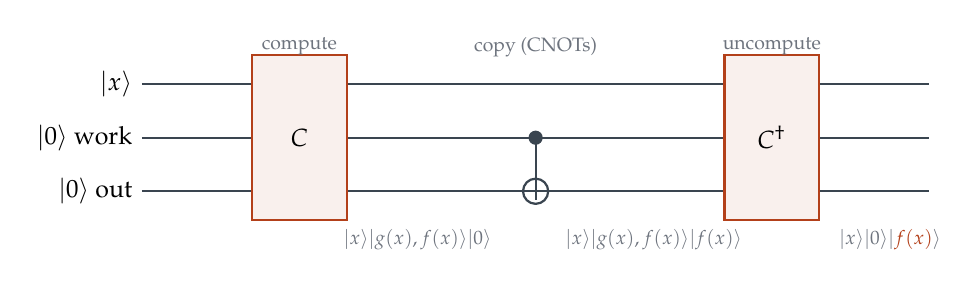
\begin{tikzpicture}[x=10mm,y=6.8mm]
    \foreach \y/\l in {2/{$|x\rangle$},1/{$|0\rangle$ work},0/{$|0\rangle$ out}} {
      \node[lab] at (0,\y) {\l}; \draw[wire] (0,\y) -- (10,\y);}
    \node[op,minimum height=21mm,minimum width=12mm] at (2,1) {$C$};
    \draw[thick,color=body] (5,1) -- (5,0); \node[dot] at (5,1) {}; \oplusat{5}{0}
    \node[op,minimum height=21mm,minimum width=12mm] at (8,1) {$C^\dagger$};
    \node[note] at (3.5,-0.9) {$|x\rangle|g(x),f(x)\rangle|0\rangle$};
    \node[note] at (6.5,-0.9) {$|x\rangle|g(x),f(x)\rangle|f(x)\rangle$};
    \node[note] at (9.5,-0.9) {$|x\rangle|0\rangle|\tgt{f(x)}\rangle$};
    \node[note] at (2,2.7) {compute}; \node[note] at (5,2.7) {copy (CNOTs)}; \node[note] at (8,2.7) {uncompute};
  \end{tikzpicture}
  \vskip2mm
  \begin{columns}[T]
    \begin{column}{0.47\textwidth}
      \blocktitle{The price}
      About twice the gates, plus a register for the copy. That factor 2 is in every count that follows.
    \end{column}
    \begin{column}{0.47\textwidth}
      \blocktitle{Where it returns}
      the modular adder's flag $\cdot$ multiply, swap, \emph{un}-multiply $\cdot$ the second division of a point addition $\cdot$ the temporary AND
    \end{column}
  \end{columns}
  \resolved{Every scratch register must be back in $|0\rangle$ before the QFT. Bennett's pattern does it, at the price of running the computation backwards.}
\end{frame}

% =====================================================================================
\act{Act IV --- building the factoring circuit, level by level}

\begin{frame}[fragile]{Act IV --- Qiskit in a few idioms}
  \begin{columns}[T]
    \begin{column}{0.64\textwidth}
      \code[basicstyle=\ttfamily\fontsize{7.2}{8.4}\selectfont]{qiskit_idioms.py}
    \end{column}
    \begin{column}{0.32\textwidth}
      \small
      prints \texttt{\{'011': 100\}}
      \vskip2mm
      \blocktitle{Idioms used throughout}
      \textbf{builders}: functions that append gates to a circuit\par
      \texttt{mcx}, \texttt{mcp}: multi-controlled $X$ and phase\par
      \texttt{.inverse()}: run backwards --- uncomputation\par
      \texttt{to\_gate()}: a sub-circuit as one box\par
      counts: bit strings, \textbf{qubit 0 rightmost}
    \end{column}
  \end{columns}
\end{frame}

\begin{frame}{Five levels, each a product of the one below}
  \begin{difficulty}{4}How does ``multiply by $a$ modulo $N$'' become gates? Build it in levels, and check each level exactly before using it.\end{difficulty}
  \centering
  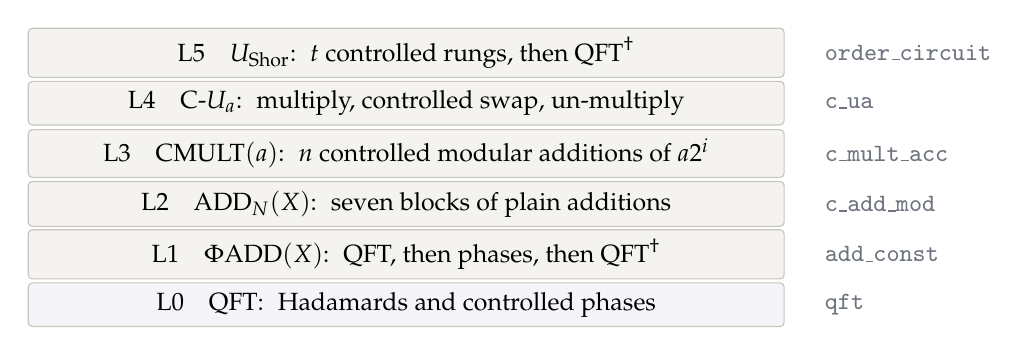
\begin{tikzpicture}[lvl/.style={draw=rulegrey,fill=greybox,rounded corners=1.5pt,minimum width=96mm,
        minimum height=5.3mm,font=\small,anchor=west},
      fn/.style={font=\ttfamily\small,color=subtle,anchor=west}]
    \foreach \i/\l/\f/\c in {
        5/{L5\quad $U_{\text{Shor}}$: \ $t$ controlled rungs, then $\mathrm{QFT}^\dagger$}/order\_circuit/greybox,
        4/{L4\quad $\text{C-}U_a$: \ multiply, controlled swap, un-multiply}/c\_ua/greybox,
        3/{L3\quad $\mathrm{CMULT}(a)$: \ $n$ controlled modular additions of $a2^i$}/c\_mult\_acc/greybox,
        2/{L2\quad $\mathrm{ADD}_N(X)$: \ seven blocks of plain additions}/c\_add\_mod/greybox,
        1/{L1\quad $\Phi\mathrm{ADD}(X)$: \ QFT, then phases, then $\mathrm{QFT}^\dagger$}/add\_const/greybox,
        0/{L0\quad $\mathrm{QFT}$: \ Hadamards and controlled phases}/qft/lavender} {
      \node[lvl,fill=\c] at (0,0.64*\i) {\l};
      \node[fn] at (10,0.64*\i) {\f};}
  \end{tikzpicture}
  \begin{takeaway}Each level is verified exhaustively --- every input, every ancilla back to $|0\rangle$ --- before the next is built on it.\end{takeaway}
\end{frame}

\begin{frame}{L0 --- the QFT is Hadamards and controlled phases}
  \vskip-2mm
  \[
    \mathrm{QFT}|j\rangle=\bigotimes_{q=0}^{n-1}\frac{|0\rangle+e^{2\pi i\,j2^q/2^n}|1\rangle}{\sqrt2}
    \quad\Longrightarrow\quad
    \mathrm{QFT}=\mathrm{SWAP}_{\text{rev}}\,B_0\cdots B_{n-1}
  \]
  \vskip-2mm
  \[ B_j=\Big(\prod_{k<j}\mathrm{CP}\big(\tfrac{\pi}{2^{j-k}}\big)\Big)H_j \]
  \begin{columns}[c]
    \begin{column}{0.52\textwidth}
      \centering\fig[width=0.92\textwidth]{qft3.pdf}
    \end{column}
    \begin{column}{0.44\textwidth}
      The output is a product state: one Hadamard per qubit, and one controlled phase per lower bit.
      \vskip2mm
      {\small $n$ Hadamards, $n(n-1)/2$ controlled phases, $\lfloor n/2\rfloor$ swaps. The swaps only undo a bit reversal (3 CNOT, 0 T).}
    \end{column}
  \end{columns}
\end{frame}

\begin{frame}[fragile]{L0 in Qiskit}
  \begin{columns}[T]
    \begin{column}{0.66\textwidth}
      \code[basicstyle=\ttfamily\scriptsize]{qft.py}
    \end{column}
    \begin{column}{0.3\textwidth}
      \blocktitle{Checked}
      equal to the DFT matrix, and to Qiskit's \texttt{QFTGate}, for $n=1,\dots,6$.
      \vskip2mm
      \blocktitle{Its cost}
      $\mathrm{CP}(\pi/2)$ is exact (3 T). The other controlled phases hold small rotations: $3\binom{n-1}{2}$ per QFT.
    \end{column}
  \end{columns}
  \begin{takeaway}\texttt{approx} drops the smallest rotations: the approximate QFT of Act VII.\end{takeaway}
\end{frame}

\begin{frame}{L1 --- Draper's adder: addition is a phase}
  In the Fourier basis, qubit $i$ of $\mathrm{QFT}|y\rangle$ carries $e^{2\pi i\,y2^i/2^m}$. Adding $X$ multiplies it by $e^{2\pi i\,X2^i/2^m}$: one phase per qubit, \textbf{no carries}.
  \[
    \Phi\mathrm{ADD}(X)=\mathrm{QFT}^\dagger\Big(\bigotimes_{i=0}^{m-1}P\big(2\pi X2^{i}/2^{m}\big)\Big)\,\mathrm{QFT}
  \]
  \centering\fig[width=0.27\textwidth]{draper3.pdf}\par
  {\scriptsize\color{subtle}$X=3$ on 3 qubits: checked equal to the cyclic shift $y\mapsto y+3 \bmod 8$.}
  \begin{takeaway}To control the adder, control only the phases: the QFT pair cancels when they do not fire.\end{takeaway}
\end{frame}

\begin{frame}{L2 --- the modular adder in seven blocks}
  \centering
  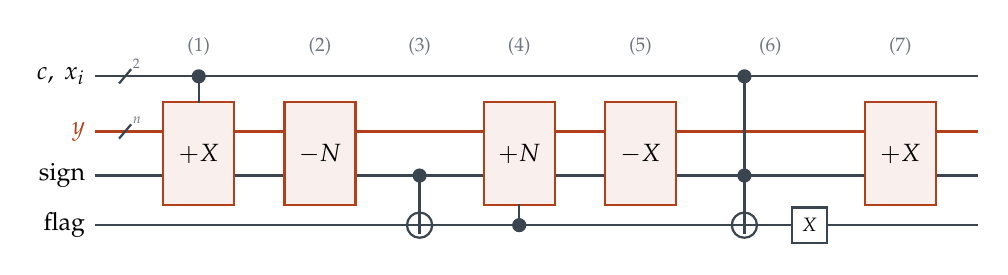
\begin{tikzpicture}[x=11mm,y=7mm]
    \node[lab] at (0,3) {$c,\ x_i$}; \draw[wire] (0,3) -- (10.2,3); \bundle{0.35}{3}{2}
    \node[lab,color=cverm] at (0,2) {$y$}; \draw[twire] (0,2) -- (10.2,2); \bundle{0.35}{2}{$n$}
    \node[lab] at (0,1.2) {sign}; \draw[wire] (0,1.2) -- (10.2,1.2);
    \node[lab] at (0,0.3) {flag}; \draw[wire] (0,0.3) -- (10.2,0.3);
    \foreach \x/\l in {1.2/{$+X$},2.6/{$-N$},4.9/{$+N$},6.3/{$-X$},9.3/{$+X$}}
      \node[op,minimum width=9mm,minimum height=13mm] (b\x) at (\x,1.6) {\l};
    \draw[thick,color=body] (1.2,3) -- (1.2,2.52); \node[dot] at (1.2,3) {};
    \draw[thick,color=body] (3.75,1.2) -- (3.75,0.3); \node[dot] at (3.75,1.2) {}; \oplusat{3.75}{0.3}
    \draw[thick,color=body] (4.9,0.3) -- (4.9,0.68); \node[dot] at (4.9,0.3) {};
    \draw[thick,color=body] (7.5,3) -- (7.5,0.3); \node[dot] at (7.5,3) {}; \node[dot] at (7.5,1.2) {}; \oplusat{7.5}{0.3}
    \node[draw=body,fill=white,thick,minimum size=4.5mm,font=\scriptsize,inner sep=1pt] at (8.25,0.3) {$X$};
    \foreach \x/\l in {1.2/1,2.6/2,3.75/3,4.9/4,6.3/5,7.8/6,9.3/7} \node[note] at (\x,3.55) {(\l)};
  \end{tikzpicture}
  \vskip1mm
  \begin{columns}[T]
    \begin{column}{0.47\textwidth}
      \blocktitle{(1)--(4): add, then reduce}
      Add $X$; subtract $N$; copy the sign --- did it go negative? --- into the flag; add $N$ back if so.
    \end{column}
    \begin{column}{0.47\textwidth}
      \blocktitle{(5)--(7): uncompute the flag}
      Subtract $X$, so the sign reveals the flag; clear it; add $X$ again. Bennett, inside one adder.
    \end{column}
  \end{columns}
  \begin{takeaway}Only blocks (1) and (6) carry the outer controls: the others cancel in pairs when the controls are off.\end{takeaway}
\end{frame}

\begin{frame}{L3--4 --- multiply, swap, un-multiply}
  Shift-and-add, $ax=\sum_i x_i\,(a2^i)$, gives an \emph{out-of-place} product: \ $\mathrm{CMULT}(a)$ is $n$ modular additions of $a2^i$, each controlled by $c$ and $x_i$. Phase estimation needs $U_a$ \emph{in place}:
  \vskip2mm
  \centering
  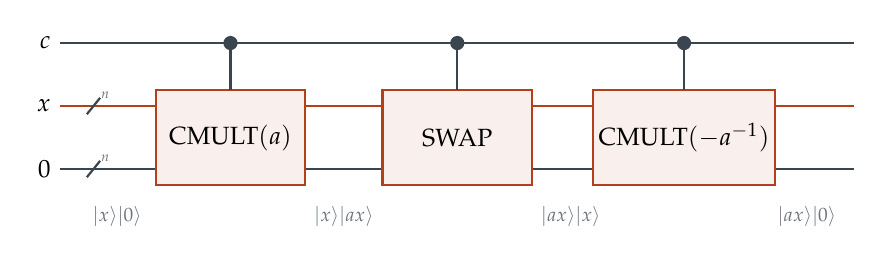
\begin{tikzpicture}[x=12mm,y=8mm]
    \node[lab] at (0,2.2) {$c$}; \draw[wire] (0,2.2) -- (8.4,2.2);
    \node[lab] at (0,1.2) {$x$}; \draw[twire] (0,1.2) -- (8.4,1.2); \bundle{0.35}{1.2}{$n$}
    \node[lab] at (0,0.2) {$0$}; \draw[wire] (0,0.2) -- (8.4,0.2); \bundle{0.35}{0.2}{$n$}
    \foreach \x/\l in {1.8/{$\mathrm{CMULT}(a)$},4.2/{SWAP},6.6/{$\mathrm{CMULT}(-a^{-1})$}} {
      \node[op,minimum width=19mm,minimum height=12mm] at (\x,0.7) {\l};
      \draw[thick,color=body] (\x,2.2) -- (\x,1.46); \node[dot] at (\x,2.2) {};}
    \node[note] at (0.6,-0.55) {$|x\rangle|0\rangle$};
    \node[note] at (3.0,-0.55) {$|x\rangle|ax\rangle$};
    \node[note] at (5.4,-0.55) {$|ax\rangle|x\rangle$};
    \node[note] at (7.9,-0.55) {$|ax\rangle|0\rangle$};
  \end{tikzpicture}
  \vskip1mm
  \raggedright
  \[ \text{C-}U_a=\mathrm{CMULT}(-a^{-1})\cdot\text{C-SWAP}\cdot\mathrm{CMULT}(a) \]
  \begin{takeaway}One rung is $2n$ modular additions and $n$ controlled swaps. The second multiplication only erases the input: uncomputation, made possible by $a^{-1}$.\end{takeaway}
\end{frame}

\begin{frame}[fragile]{L3--4 in Qiskit}
  \begin{columns}[T]
    \begin{column}{0.7\textwidth}
      \code[basicstyle=\ttfamily\scriptsize]{c_ua.py}
    \end{column}
    \begin{column}{0.27\textwidth}
      \blocktitle{Why the inverse exists}
      $\gcd(a,N)=1$, so $a^{-1}\bmod N$ exists; it is computed classically.
      \vskip2mm
      \blocktitle{Checked}
      $|x\rangle|0\rangle\mapsto|ax \bmod N\rangle|0\rangle$ for every $x$, every $a$ coprime to $N$, both control values.
    \end{column}
  \end{columns}
\end{frame}

\begin{frame}{L5 --- the whole circuit, $N=15$, $a=7$}
  \centering
  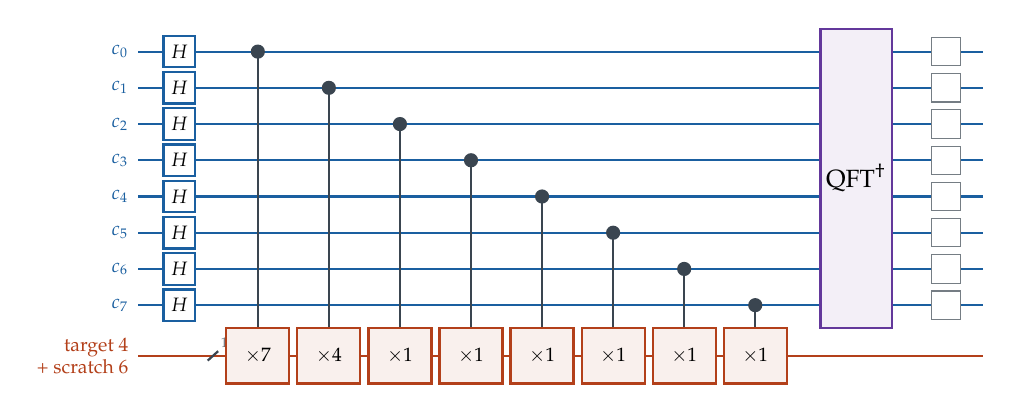
\begin{tikzpicture}[x=9.5mm,y=4.6mm]
    \foreach \i in {0,...,7} {
      \pgfmathsetmacro{\yy}{7-\i}
      \node[lab,color=cblue,font=\scriptsize] at (0,\yy) {$c_{\i}$};
      \draw[cwire] (0,\yy) -- (11.3,\yy);
      \node[hop,minimum size=4mm,font=\scriptsize] at (0.55,\yy) {$H$};}
    \node[lab,color=cverm,font=\scriptsize,align=right] at (0,-1.4) {target 4\\+ scratch 6};
    \draw[twire] (0,-1.4) -- (11.3,-1.4); \bundle{1.0}{-1.4}{10}
    \foreach \i/\m in {0/7,1/4,2/1,3/1,4/1,5/1,6/1,7/1} {
      \pgfmathsetmacro{\xx}{1.6+0.95*\i}
      \pgfmathsetmacro{\yy}{7-\i}
      \draw[thick,color=body] (\xx,\yy) -- (\xx,-0.95);
      \node[dot] at (\xx,\yy) {};
      \node[op,minimum width=8mm,minimum height=7mm,font=\scriptsize] at (\xx,-1.4) {$\times\m$};}
    \node[qop,minimum height=38mm,minimum width=9mm] at (9.6,3.5) {$\mathrm{QFT}^\dagger$};
    \foreach \i in {0,...,7} \node[meter,minimum size=3.6mm] at (10.8,\i) {};
  \end{tikzpicture}
  \vskip1mm
  \begin{columns}[T]
    \begin{column}{0.47\textwidth}
      \blocktitle{$4n+2=18$ qubits}
      \cnt{8 counting}, \tgt{4 target}, 4 scratch, sign and flag.
    \end{column}
    \begin{column}{0.47\textwidth}
      {\small Rung $i$ multiplies by $7^{2^i}\bmod15$: $7,4,1,1,\dots$ The circuit keeps the $\times1$ rungs --- skipping them would use $r$ to build the circuit that finds $r$.}
    \end{column}
  \end{columns}
\end{frame}

\begin{frame}[fragile]{L5 in Qiskit}
  \begin{columns}[T]
    \begin{column}{0.7\textwidth}
      \code[basicstyle=\ttfamily\scriptsize]{order_circuit.py}
    \end{column}
    \begin{column}{0.27\textwidth}
      \blocktitle{Five short functions}
      \texttt{qft}, \texttt{add\_const}, \texttt{c\_add\_mod}, \texttt{c\_ua}, \texttt{order\_circuit} --- each a product of the one before --- make the complete order-finding circuit.
    \end{column}
  \end{columns}
  \resolved{The box is modular multiplication, built from Fourier adders, with uncomputation at two levels. Next: run it.}
\end{frame}

% =====================================================================================
\act{Act V --- simulation, and reading the answer}

\begin{frame}[fragile]{Act V --- running it on Aer}
  \begin{difficulty}{5}The measurement returns one integer $y$. How is $r$ read from it, and how do we know the circuit is right?\end{difficulty}
    \code[basicstyle=\ttfamily\scriptsize]{run_aer.py}
  {\small prints \texttt{18 4}: 18 qubits, order $r=4$. \ \texttt{transpile} rewrites the circuit into the simulator's gate set; 4096 shots take about 2 s.}
\end{frame}

\begin{frame}{$N=15$: four sharp peaks}
  \begin{columns}[c]
    \begin{column}{0.5\textwidth}
      \centering\fig[width=\textwidth]{n15_hist.pdf}
    \end{column}
    \begin{column}{0.46\textwidth}
      \blocktitle{The exact distribution}
      The target takes $r$ values, one per residue $x_0=x \bmod r$:
      \[ P(y)=\frac{1}{4^{t}}\sum_{x_0<r}\Big|\sum_{m} e^{-2\pi i\,m r y/2^t}\Big|^2 \]
      Aer's exact probabilities equal it.
    \end{column}
  \end{columns}
  \vskip1mm
  {\small \textbf{Samples vs exact:} the total variation distance $\tfrac12\sum_y|\hat p(y)-p(y)|$ is $0.006$. A perfect sampler exceeds $0.032$ only 0.01\% of the time at 4096 shots --- the \emph{shot-noise bound}.}
\end{frame}

\begin{frame}{From $y$ to $r$ to the factors}
  Each peak is $y\approx 2^t\,s/\per{r}$. Continued fractions give $s/r$ in lowest terms; its denominator is a candidate $r$, checked with $a^r\equiv1$.
  \vskip2mm
  \begin{columns}[T]
    \begin{column}{0.52\textwidth}
      \centering\small
      \begin{tabular}{rrcc}
        \toprule
        $y$ & shots & $y/2^8$ & candidate $r$ \\
        \midrule
        64 & 1037 & $1/4$ & \textbf{4} \ \checkmark \\
        128 & 1037 & $1/2$ & 2 \ ($7^2\not\equiv1$) \\
        192 & 1015 & $3/4$ & \textbf{4} \ \checkmark \\
        0 & 1007 & $0$ & --- \\
        \bottomrule
      \end{tabular}
    \end{column}
    \begin{column}{0.44\textwidth}
      \begin{greyblock}
        \blocktitle{Then Euclid}
        $r=4$, and $7^2=49\equiv4\not\equiv-1$:\par
        $\gcd(7^2-1,15)=3$,\ \ $\gcd(7^2+1,15)=5$.
      \end{greyblock}
    \end{column}
  \end{columns}
  \begin{takeaway}One shot gives $r$ with probability $1/2$ here (measured $0.501$): about two runs expected. A failed shot costs a run, never a wrong answer.\end{takeaway}
\end{frame}

\begin{frame}[fragile]{Post-processing in code}
  \begin{columns}[T]
    \begin{column}{0.64\textwidth}
      \code[basicstyle=\ttfamily\scriptsize]{order_from_counts.py}
    \end{column}
    \begin{column}{0.33\textwidth}
      \blocktitle{Continued fractions in one call}
      \texttt{limit\_denominator(N-1)} returns the best fraction with denominator $<N$: the continued-fraction convergent.
      \vskip2mm
      \blocktitle{Failure modes, all caught}
      $y=0$ or $\gcd(s,r)>1$: a divisor of $r$ --- take another shot. $r$ odd or $a^{r/2}\equiv-1$: pick another $a$ (probability $\le1/2$).
    \end{column}
  \end{columns}
\end{frame}

\begin{frame}{When $r$ does not divide $2^t$: $N=21$, $a=2$, $r=6$}
  \centering\fig[width=0.92\textwidth]{n21_exact.pdf}
  \begin{columns}[T]
    \begin{column}{0.47\textwidth}
      \blocktitle{Continued fractions at work}
      $y=171$: \ $\dfrac{171}{1024}=[0;5,1,84,2]$, convergents $\tfrac15,\ \tfrac16,\dots$ \ $\tfrac16$ gives $r=6$, and $2^6\equiv1 \pmod{21}$.
    \end{column}
    \begin{column}{0.47\textwidth}
      \blocktitle{Why $t=2n$}
      Legendre: if $|y/2^t-s/r|<1/(2r^2)$, then $s/r$ is a convergent; $2^t\ge N^2$ guarantees it. The peaks smear: $P=0.322$ per shot.
    \end{column}
  \end{columns}
\end{frame}

% =====================================================================================
\act{Act VI --- counting qubits, Toffolis and T gates}

\begin{frame}{Act VI --- the counts follow from the construction}
  \begin{difficulty}{6}How many qubits and gates does the circuit need, and which of them dominate the fault-tolerant cost?\end{difficulty}
  \centering\small
  \renewcommand{\arraystretch}{1.2}
  \begin{tabular}{llll}
    \toprule
    level & qubits & Toffoli & controlled phases \\
    \midrule
    controlled $\mathrm{ADD}_N$ (10 QFTs, $m=n+1$) & $n+4$ & $2m+3$ & $5m(m-1)+2m$ \\
    one rung $\text{C-}U_a$ & $2n+3$ & $4n^2+11n$ & $2n\,(5m(m-1)+2m)$ \\
    $U_{\text{Shor}}$: $2n$ rungs $+\,\mathrm{QFT}^\dagger$ & $\mathbf{4n+2}$ & $\mathbf{8n^3+22n^2}$ & $\approx\mathbf{20\,n^4}$ \\
    \bottomrule
  \end{tabular}
  \vskip2mm
  \raggedright
  {\small Toffolis: $2n$ rungs $\times$ \big($2n$ additions $\times(2m+3)$ + $n$ controlled swaps\big) $=8n^3+22n^2$. They come from the doubly-controlled phases (2 each) and one triply-controlled NOT per addition (3).}
  \begin{takeaway}$O(n)$ qubits, $O(n^3)$ Toffolis --- and $O(n^4)$ controlled phases. Every count equals its formula exactly for $n=4,\dots,8$ (backup).\end{takeaway}
\end{frame}

\begin{frame}{$N=15$: where the T gates go}
  \begin{columns}[c]
    \begin{column}{0.54\textwidth}
      \begin{greyblock}
        \blocktitle{Exact in Clifford+T}
        864 Toffolis \hfill 6\,048 T\par
        $\pi/4$ phases (CS, T) \hfill 8\,261 T\par
      \end{greyblock}
      \begin{peachblock}
        \peachtitle{To be synthesised}
        12\,855 small rotations \hfill $\approx$ 964\,000 T\par
      \end{peachblock}
      \textbf{Total $\approx$ 978\,000 T: 98.5\% from rotations.}
    \end{column}
    \begin{column}{0.42\textwidth}
      \small
      Counted by \texttt{resources.count}, which walks the circuit and prices each gate by its standard decomposition.
      \vskip2mm
      Each of the $R$ rotations is synthesised to error $10^{-3}/R$: $\approx3\log_2(R/10^{-3})$ T each.
    \end{column}
  \end{columns}
  \begin{takeaway}The Toffolis are not the problem. The rotations of the Fourier arithmetic are.\end{takeaway}
\end{frame}

\begin{frame}{At RSA-2048 size}
  \begin{columns}[T]
    \begin{column}{0.47\textwidth}
      \begin{peachblock}
        \peachtitle{This circuit, from the verified formulas}
        8\,194 qubits,\ \ $6.9\times10^{10}$ Toffolis\par
        exact QFTs: $\approx2\times10^{17}$ T\par
        approximate QFTs: $\approx1\times10^{16}$ T\par
        \vskip1mm
        {\small still dominated by rotations}
      \end{peachblock}
    \end{column}
    \begin{column}{0.47\textwidth}
      \begin{greyblock}
        \blocktitle{Reported by the state of the art}
        Gidney--Ekerå 2021: $\approx6\,200$ qubits, $2.7\times10^{9}$ Toffolis --- ripple-carry, windowed.\par
        \vskip1mm
        Gidney 2025: $\approx1\,400$ qubits, $6.5\times10^{9}$ Toffolis per run --- approximate residue arithmetic.
      \end{greyblock}
    \end{column}
  \end{columns}
  \resolved{The textbook circuit is polynomial but enormous, and most of its cost is rotations. The optimisations of Act VII remove them first.}
\end{frame}

% =====================================================================================
\act{Act VII --- the optimisations, one idea each}

\begin{frame}{Act VII --- what each optimisation removes}
  \begin{difficulty}{7}Which parts of the textbook circuit are expensive, and what replaces them?\end{difficulty}
  \centering
  \renewcommand{\arraystretch}{1.25}
  \begin{tabular}{lll}
    \toprule
    optimisation & removes & measured effect \\
    \midrule
    semiclassical QFT & the counting register & $4n+2\to2n+3$ qubits \\
    ripple-carry adder & all rotations in the arithmetic & T $\div19$ ($n=4$) \dots\ $\div99$ ($n=12$) \\
    temporary AND & the T cost of uncomputing & 14 T $\to$ 4 T per pair \\
    windowing & most modular additions & $n\to\lceil n/w\rceil$ per multiply \\
    approximate QFT & the smallest rotations & $-34\%$ rotations ($n=8$), lossy \\
    \bottomrule
  \end{tabular}
  \vskip2mm
  {\small All implemented and verified in \texttt{shor\_qiskit/}. The coset representation and measurement-based uncomputation are in the backup.}
\end{frame}

\begin{frame}{One counting qubit: the semiclassical QFT}
  Every rotation of $\mathrm{QFT}^\dagger$ is controlled by a qubit that is \emph{about to be measured}. Measure it first and control classically: the distribution is unchanged (deferred measurement).
  \vskip1mm
  \centering
  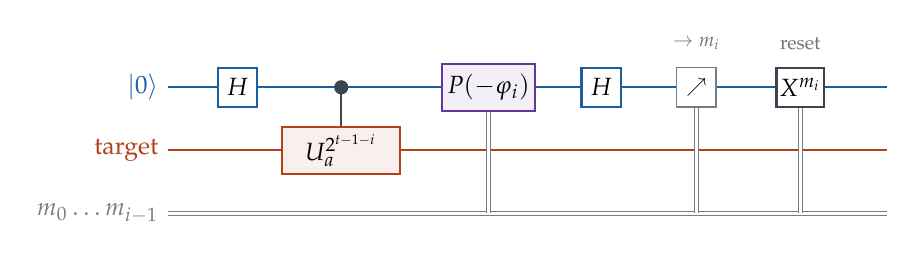
\begin{tikzpicture}[x=11mm,y=8mm]
    \node[lab,color=cblue] at (0,1.6) {$|0\rangle$}; \draw[cwire] (0,1.6) -- (8.3,1.6);
    \node[lab,color=cverm] at (0,0.6) {target}; \draw[twire] (0,0.6) -- (8.3,0.6);
    \node[lab,color=quotebar] at (0,-0.4) {$m_0\dots m_{i-1}$}; \draw[clw] (0,-0.4) -- (8.3,-0.4);
    \node[hop] at (0.8,1.6) {$H$};
    \draw[thick,color=body] (2.0,1.6) -- (2.0,0.9); \node[dot] at (2.0,1.6) {};
    \node[op,minimum width=15mm,minimum height=6mm] at (2.0,0.6) {$U_a^{2^{t-1-i}}$};
    \node[qop,minimum height=6mm] (ph) at (3.7,1.6) {$P(-\varphi_i)$};
    \draw[clw] (3.7,-0.4) -- (ph.south);
    \node[hop] at (5.0,1.6) {$H$};
    \node[meter] (m) at (6.1,1.6) {$\nearrow$};
    \draw[clw] (m.south) -- (6.1,-0.4);
    \node[draw=body,fill=white,thick,minimum size=5mm,font=\small,inner sep=1pt] (x) at (7.3,1.6) {$X^{m_i}$};
    \draw[clw] (7.3,-0.4) -- (x.south);
    \node[note] at (6.1,2.3) {$\to m_i$}; \node[note] at (7.3,2.3) {reset};
  \end{tikzpicture}
  \[ \varphi_i=\pi\sum_{j<i} m_j/2^{\,i-j},\qquad \text{repeat for } i=0,\dots,t-1 \ \text{(heaviest rung first)} \]
  \begin{takeaway}One recycled qubit replaces all $2n$ counting qubits: $4n+2\to2n+3$. The controlled phases become classically controlled single-qubit phases.\end{takeaway}
\end{frame}

\begin{frame}{In Qiskit: a dynamic circuit}
  \centering\fig[width=0.74\textwidth]{semiclassical_phase.pdf}\par
  {\scriptsize\color{subtle}The loop on its own, with phase gates as the rungs ($y=5$, $t=3$): Aer reads back \texttt{101} on every shot.}
  \vskip2mm
  \raggedright
  \texttt{if\_test} is \textbf{mid-circuit measurement and feed-forward}: the classical bits already measured decide which phases fire. Hardware runs this as a dynamic circuit.
\end{frame}

\begin{frame}[fragile]{The loop in code}
  \code[basicstyle=\ttfamily\scriptsize]{semiclassical.py}
  \begin{columns}[T]
    \begin{column}{0.47\textwidth}
      \blocktitle{One loop, both problems}
      The rungs are callbacks: the same function drives factoring and ECDLP.
    \end{column}
    \begin{column}{0.47\textwidth}
      \blocktitle{Checked exactly}
      Enumerating the measurement branches, its distribution equals the full circuit's to $10^{-13}$.
    \end{column}
  \end{columns}
\end{frame}

\begin{frame}{$N=21$ on 13 qubits instead of 22}
  \centering\fig[width=0.97\textwidth]{n21_measured.pdf}\par
  {\scriptsize\color{subtle}bars: Aer, 1024 shots of the one-counting-qubit circuit; dots: the exact distribution around each peak $s\cdot2^{10}/6$.}
  \vskip2mm
  \begin{columns}[T]
    \begin{column}{0.47\textwidth}
      \blocktitle{Same distribution}
      total variation distance $0.075$, within the shot-noise bound $0.108$.
    \end{column}
    \begin{column}{0.47\textwidth}
      \blocktitle{Same success}
      one shot gives $r=6$ with probability $0.322$ exact, $0.313$ measured; $21=7\times3$.
    \end{column}
  \end{columns}
\end{frame}

\begin{frame}{Toffoli arithmetic: the ripple-carry adder}
  \begin{columns}[c]
    \begin{column}{0.46\textwidth}
      \centering\fig[width=0.95\textwidth]{rc_adder.pdf}
    \end{column}
    \begin{column}{0.5\textwidth}
      Cuccaro et al.: \textbf{MAJ} blocks carry up, \textbf{UMA} blocks write the sum on the way down. Each is one Toffoli and two CNOTs.
      \vskip2mm
      \begin{greyblock}
        $2m$ Toffolis, one carry qubit, \textbf{no rotations}. The seven blocks of the modular adder stay the same; only the adder inside changes.
      \end{greyblock}
    \end{column}
  \end{columns}
\end{frame}

\begin{frame}{Toffolis are cheaper than rotations}
  \begin{columns}[c]
    \begin{column}{0.52\textwidth}
      \centering\fig[width=\textwidth]{rung_T.pdf}
    \end{column}
    \begin{column}{0.44\textwidth}
      One rung, T gates with every rotation synthesised.
      \vskip2mm
      \begin{greyblock}
        Ripple-carry: 7--8$\times$ \textbf{more} Toffolis, but no rotations.\par
        T: $\div19$ at $n=4$, $\div99$ at $n=12$.
      \end{greyblock}
      {\small The gap grows like $n$: rotations scale as $n^4$, Toffolis as $n^3$.}
    \end{column}
  \end{columns}
\end{frame}

\begin{frame}{The temporary AND: uncomputation for free}
  \centering\fig[width=0.74\textwidth]{and_gadget.pdf}\par
  {\scriptsize\color{subtle}Compute with 4 T; uncompute by an $X$-basis measurement and a classically controlled CZ.}
  \vskip1mm
  \begin{columns}[T]
    \begin{column}{0.47\textwidth}
      \blocktitle{Why it works}
      The target starts in $|0\rangle$: 4 T, not 7. An $X$-basis measurement reveals nothing about $a,b$; a Clifford fixes the phase.
    \end{column}
    \begin{column}{0.47\textwidth}
      \blocktitle{What it saves}
      A compute/uncompute pair drops from 14 T to 4: a table lookup costs $3.5\times$ fewer T.
    \end{column}
  \end{columns}
\end{frame}

\begin{frame}{Windowing: look the answer up, then add once}
  Take $w$ bits $j$ of $x$ at a time, and \textbf{look up} their contribution $T[j]=a\,j\,2^i\bmod N$ from a classical table:
  \vskip1mm
  \centering
  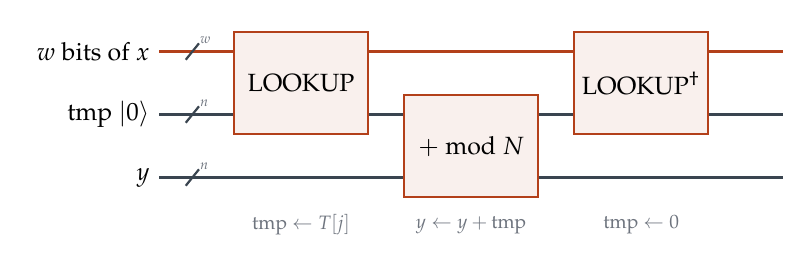
\begin{tikzpicture}[x=12mm,y=8mm]
    \node[lab] at (0,2) {$w$ bits of $x$}; \draw[twire] (0,2) -- (6.6,2); \bundle{0.35}{2}{$w$}
    \node[lab] at (0,1) {tmp $|0\rangle$}; \draw[wire] (0,1) -- (6.6,1); \bundle{0.35}{1}{$n$}
    \node[lab] at (0,0) {$y$}; \draw[wire] (0,0) -- (6.6,0); \bundle{0.35}{0}{$n$}
    \node[op,minimum width=17mm,minimum height=13mm] at (1.5,1.5) {LOOKUP};
    \node[op,minimum width=17mm,minimum height=13mm] at (3.3,0.5) {$+$ mod $N$};
    \node[op,minimum width=17mm,minimum height=13mm] at (5.1,1.5) {LOOKUP$^\dagger$};
    \node[note] at (1.5,-0.75) {tmp $\leftarrow T[j]$}; \node[note] at (3.3,-0.75) {$y\leftarrow y+\text{tmp}$}; \node[note] at (5.1,-0.75) {tmp $\leftarrow0$};
  \end{tikzpicture}
  \vskip1mm
  \raggedright
  \begin{columns}[T]
    \begin{column}{0.47\textwidth}
      {\small The lookup is \textbf{unary iteration}: a tree of Toffolis walks the $L=2^w$ addresses, $2(L-1)$ Toffolis, and loads each entry with CNOTs.}
    \end{column}
    \begin{column}{0.47\textwidth}
      {\small $n\to\lceil n/w\rceil$ additions per multiplication. One rung at $n=12$, $w=4$: T drops from $4.0\times10^6$ to $1.2\times10^6$.}
    \end{column}
  \end{columns}
\end{frame}

\begin{frame}{Approximate QFT: fewer rotations, but errors add up}
  Drop every $\mathrm{CP}(\pi/2^k)$ with $k>d$, in every adder's QFT. On $N=15$:
  \vskip2mm
  \centering
  \renewcommand{\arraystretch}{1.2}
  \begin{tabular}{lrrr}
    \toprule
    QFTs & small rotations & distance from exact & P(one shot gives $r$) \\
    \midrule
    exact & 12\,855 & 0.006 & 0.501 \\
    $d=4$ & 12\,837 & 0.006 & 0.501 \\
    $d=3$ & 10\,905 & \textbf{0.138} & 0.451 \\
    $d=2$ & 7\,050 & \textbf{0.594} & 0.245 \\
    \bottomrule
  \end{tabular}
  \vskip2mm
  \raggedright{\small The circuit holds 320 Fourier additions, each with its own approximation error; they accumulate. The shot-noise bound is 0.032.}
  \begin{takeaway}One error budget is shared by every approximation, so $d$ must grow like $\log_2(\#\text{additions}/\varepsilon)$. At $n=8$, $d=4$ already removes a third of the rotations.\end{takeaway}
\end{frame}

\begin{frame}{All together: $N=15$}
  \centering\fig[width=0.84\textwidth]{variants.pdf}
  \vskip1mm
  \raggedright
  {\small In raw Toffolis the ripple-carry versions look $7\times$ worse; priced with synthesis they win by more than $20\times$. One counting qubit + ripple-carry: 17 qubits and 42\,600 T, against 18 qubits and 978\,000 T.}
  \resolved{Remove rotations first, then qubits, then additions. (Modern estimates also combine windowing with ripple-carry adders; not built here.)}
\end{frame}

% =====================================================================================
\act{Act VIII --- the elliptic-curve discrete logarithm}

\begin{frame}{Act VIII --- ECDSA keys are discrete logarithms}
  \begin{difficulty}{8}An ECDSA or ECDH key pair is a secret number $\per{d}$ and a public point $Q=\per{d}\,G$ on a curve. Recovering $\per{d}$ from $Q$ is the elliptic-curve discrete logarithm. Does the same circuit solve it?\end{difficulty}
  \vskip2mm
  The points $(x,y)$ with $y^2=x^3+ax+b \pmod p$, plus a point at infinity $O$, form a group. Adding two points:
  \[ \lambda=\frac{y_2-y_1}{x_2-x_1},\qquad x_3=\lambda^2-x_1-x_2,\qquad y_3=\lambda(x_1-x_3)-y_1 . \]
  \begin{takeaway}Point addition needs a modular \textbf{division}. That is the whole cost difference from factoring.\end{takeaway}
\end{frame}

\begin{frame}{A toy curve}
  \begin{columns}[c]
    \begin{column}{0.4\textwidth}
      \centering\fig[width=\textwidth]{curve_p7.pdf}
    \end{column}
    \begin{column}{0.56\textwidth}
      $y^2=x^3+5x+4$ over $\mathbb{F}_7$: nine points and $O$.
      \vskip2mm
      $kP=P+\dots+P$ ($k$ times). \ $G=(0,5)$ has order $r=5$:
      \[ G,\ 2G,\ 3G,\ 4G,\ 5G=O . \]
      The public key $Q=(0,2)=\per{4}\,G$ hides $\per{k=4}$.
    \end{column}
  \end{columns}
\end{frame}

\begin{frame}{Two registers, one accumulator}
  \centering
  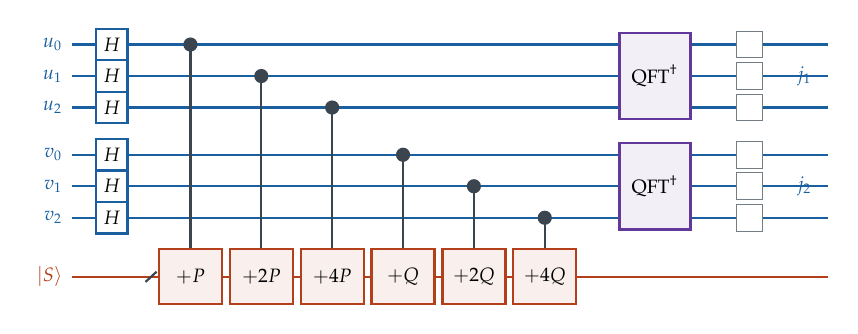
\begin{tikzpicture}[x=10mm,y=5mm]
    \foreach \y/\l in {5/u_0,4.2/u_1,3.4/u_2,2.2/v_0,1.4/v_1,0.6/v_2} {
      \node[lab,color=cblue,font=\scriptsize] at (0,\y) {$\l$};
      \draw[cwire] (0,\y) -- (9.6,\y);
      \node[hop,minimum size=4mm,font=\scriptsize] at (0.5,\y) {$H$};}
    \node[lab,color=cverm,font=\scriptsize] at (0,-0.9) {$|S\rangle$}; \draw[twire] (0,-0.9) -- (9.6,-0.9); \bundle{1.0}{-0.9}{$2n$}
    \foreach \x/\y/\l in {1.5/5/P,2.4/4.2/2P,3.3/3.4/4P,4.2/2.2/Q,5.1/1.4/2Q,6.0/0.6/4Q} {
      \draw[thick,color=body] (\x,\y) -- (\x,-0.45); \node[dot] at (\x,\y) {};
      \node[op,minimum width=8mm,minimum height=7mm,font=\scriptsize] at (\x,-0.9) {$+\l$};}
    \node[qop,minimum height=11mm,minimum width=9mm,font=\scriptsize] at (7.4,4.2) {$\mathrm{QFT}^\dagger$};
    \node[qop,minimum height=11mm,minimum width=9mm,font=\scriptsize] at (7.4,1.4) {$\mathrm{QFT}^\dagger$};
    \foreach \y in {5,4.2,3.4,2.2,1.4,0.6} \node[meter,minimum size=3.4mm] at (8.6,\y) {};
    \node[font=\scriptsize,color=cblue] at (9.3,4.2) {$j_1$}; \node[font=\scriptsize,color=cblue] at (9.3,1.4) {$j_2$};
  \end{tikzpicture}
  \[ \frac{1}{2^m}\sum_{u,v}\cnt{|u\rangle|v\rangle}\;\tgt{|S+uP+vQ\rangle}=\frac{1}{2^m}\sum_{u,v}\cnt{|u\rangle|v\rangle}\;\tgt{|S+(u+\per{k}v)P\rangle} \]
  {\small The accumulator depends on $(u,v)$ only through $u+kv\bmod r$; two inverse QFTs turn that into $(j_1,j_2)$. $S$ is a fixed start point: affine formulas cannot represent $O$, and hitting it is a rare exceptional case (probability $O(1/p)$); the toy oracle gives $O$ its own code.}
\end{frame}

\begin{frame}[fragile]{ECDLP in Qiskit}
  \code[basicstyle=\ttfamily\fontsize{7.2}{8.3}\selectfont]{ecdlp_builder.py}
  {\small Table oracle: a permutation of the toy curve's points (12 qubits, on Aer; equals the library). Arithmetic oracle: 69 qubits, checked on every basis state.}
\end{frame}

\begin{frame}{On Aer: the key comes out}
  \centering\fig[width=0.48\textwidth]{ecdlp_heat.pdf}
  \vskip1mm
  \begin{columns}[T]
    \begin{column}{0.47\textwidth}
      \blocktitle{Same distribution}
      distance from exact $0.031$ (bound $0.054$). One shot yields $k$ with probability $0.611$ (measured $0.610$).
    \end{column}
    \begin{column}{0.47\textwidth}
      \blocktitle{Same one-qubit trick}
      With the semiclassical QFT both registers share one qubit: on a 13-point curve mod 11, $k=9$ recovered on 9 qubits instead of 16.
    \end{column}
  \end{columns}
\end{frame}

\begin{frame}{Post-processing: the key from $(j_1,j_2)$}
  \begin{columns}[c]
    \begin{column}{0.54\textwidth}
      A peak satisfies $\;j_2\,r/2^m \equiv \per{k}\,(j_1\,r/2^m) \pmod r$. Round, and divide:
      \[ a_i=\mathrm{round}\big(j_i\,r/2^m\big),\qquad \per{k}=a_2\,a_1^{-1}\bmod r . \]
      Every shot votes; the winner is checked with $kG=Q$.
      \vskip2mm
      {\small Code: \texttt{ec\_classical.ecdlp\_postprocess} (backup). It also tries $\pm1$ around the rounding when $2^m$ is not a multiple of $r$ (Ekerå).}
    \end{column}
    \begin{column}{0.42\textwidth}
      \centering\fig[width=\textwidth]{ecdlp_votes.pdf}
    \end{column}
  \end{columns}
  \begin{takeaway}$k=4$ takes 42\% of the vote, against 13--16\% for each wrong key: a signal, not luck.\end{takeaway}
\end{frame}

\begin{frame}{One point addition is eleven reversible steps}
  \begin{columns}[c]
    \begin{column}{0.54\textwidth}
      \centering\fig[width=\textwidth]{padd_steps.pdf}
    \end{column}
    \begin{column}{0.42\textwidth}
      \blocktitle{In place, no garbage}
      Step 3 divides to get $\lambda$. Step 4 clears $y$, since $x\lambda=y$. Step 8 is the \emph{same} division; by then $y/x=\lambda$ again, so it \textbf{clears} $\lambda$ --- uncomputation.
      \vskip2mm
      {\small A division is Kaliski's binary extended-Euclid inversion: $2n$ rounds of shifts and subtractions.}
    \end{column}
  \end{columns}
  \begin{takeaway}The two divisions are 80\% of the 2\,744 Toffolis of one addition ($p=7$).\end{takeaway}
\end{frame}

\begin{frame}{ECDLP costs: $O(n^2)$ per addition, $O(n^3)$ overall}
  \begin{columns}[c]
    \begin{column}{0.5\textwidth}
      \centering\fig[width=\textwidth]{ecdlp_scaling.pdf}
    \end{column}
    \begin{column}{0.46\textwidth}
      \blocktitle{Why}
      A division: $2n$ rounds of $O(n)$ Toffolis. One addition: $O(n^2)$ (measured slope 1.9). Shor adds one point per bit of $u$ and $v$: $2n$ additions, $\mathbf{O(n^3)}$ Toffolis on $O(n)$ qubits.
      \vskip2mm
      \blocktitle{No rotations}
      The arithmetic is Toffolis and CNOTs only. The inverse QFTs become classically controlled phases.
    \end{column}
  \end{columns}
\end{frame}

\begin{frame}{ECDLP optimisations, measured}
  \begin{columns}[c]
    \begin{column}{0.62\textwidth}
      \centering\fig[width=\textwidth]{ablation.pdf}
    \end{column}
    \begin{column}{0.34\textwidth}
      \small
      From eprint 2026/106 and 2026/1128, each on a fixed task, correctness re-checked.
      \vskip2mm
      Pseudo-Mersenne doubling is approximate (3\% failures). Jacobian coordinates avoid the division but leave $3n$ garbage qubits per addition. The carry-save multiplier trades $4\times$ the qubits for depth.
    \end{column}
  \end{columns}
  \resolved{The same circuit solves the ECDLP. Its box, a point addition, is costlier than a multiplication because of the division --- and again all Toffolis.}
\end{frame}

% =====================================================================================
\act{Act IX --- why ECDSA falls before RSA at the same security}

\begin{frame}{Act IX --- what an attacker must solve}
  \begin{difficulty}{9}RSA-3072 and ECDSA on P-256 are rated equally secure against classical computers. Are they equally hard for Shor?\end{difficulty}
  \vskip1mm
  \begin{columns}[T]
    \begin{column}{0.47\textwidth}
      \begin{greyblock}
        \blocktitle{RSA}
        public key $(N,e)$ with $N=pq$\par
        factor $N$ $\Rightarrow$ private exponent $d$\par
        Shor: order finding, $n=\log_2N$ bits
      \end{greyblock}
    \end{column}
    \begin{column}{0.47\textwidth}
      \begin{greyblock}
        \blocktitle{ECDSA / ECDH}
        public key $Q=dG$ on a curve over $\mathbb{F}_p$\par
        discrete logarithm $\Rightarrow$ private key $d$\par
        Shor: two registers, $n=\log_2p$ bits
      \end{greyblock}
    \end{column}
  \end{columns}
  \begin{takeaway}Shor recovers both private keys. The question is only how much each costs.\end{takeaway}
\end{frame}

\begin{frame}{Same classical security, very different key sizes}
  \begin{columns}[T]
    \begin{column}{0.47\textwidth}
      \blocktitle{Factoring: sub-exponential}
      The number field sieve runs in $\exp\big((1.92+o(1))(\ln N)^{1/3}(\ln\ln N)^{2/3}\big)$: RSA needs long keys.
      \vskip2mm
      \blocktitle{ECDLP: exponential}
      No sieve works on a good curve; the best attack is generic --- Pollard's $\rho$, $\Theta(2^{n/2})$.
    \end{column}
    \begin{column}{0.47\textwidth}
      \centering
      \renewcommand{\arraystretch}{1.2}
      \begin{tabular}{rrr}
        \toprule
        security & RSA & curve \\
        \midrule
        112 & 2048 & 224 \\
        \textbf{128} & \textbf{3072} & \textbf{256} \\
        192 & 7680 & 384 \\
        256 & 15360 & 521 \\
        \bottomrule
      \end{tabular}\par
      {\scriptsize\color{subtle}key sizes in bits (NIST SP 800-57)}
    \end{column}
  \end{columns}
  \begin{takeaway}At matched classical security the curve key is $12\times$ shorter. That is why elliptic curves are used.\end{takeaway}
\end{frame}

\begin{frame}{The price of one group operation}
  \begin{columns}[c]
    \begin{column}{0.52\textwidth}
      \centering\fig[width=\textwidth]{group_op_cost.pdf}
    \end{column}
    \begin{column}{0.44\textwidth}
      Both attacks do $2n$ controlled group operations: $\Theta(n)$ qubits, $\Theta(n^3)$ Toffolis. Only the constant differs.
      \vskip2mm
      \begin{greyblock}
        Measured on this repo's circuits, at equal $n$: one point addition costs \textbf{6.1--6.7} controlled multiplications --- constant in $n$. The division is the price.
      \end{greyblock}
    \end{column}
  \end{columns}
\end{frame}

\begin{frame}{At 128-bit security}
  \begin{columns}[c]
    \begin{column}{0.57\textwidth}
      \centering\fig[width=\textwidth]{rsa_vs_ecc.pdf}
    \end{column}
    \begin{column}{0.4\textwidth}
      \blocktitle{Toffolis}
      $(3072/256)^3=1\,728$, and $1\,728/6.7\approx260$: \par
      this repo's circuits $\approx270\times$ fewer for P-256; minimal-width literature $148\times$; optimised literature $\approx180\times$.
      \vskip2mm
      \blocktitle{Qubits}
      depend on the construction: $2.6\times$ fewer in like-for-like circuits, but RSA-2048 now fits in $\approx1\,400$ (Gidney 2025).
    \end{column}
  \end{columns}
\end{frame}

\begin{frame}{The gap grows with security}
  \begin{columns}[c]
    \begin{column}{0.52\textwidth}
      \centering\fig[width=\textwidth]{security_scaling.pdf}
    \end{column}
    \begin{column}{0.44\textwidth}
      At $\sigma$ bits of classical security:\par
      \vskip1mm
      RSA needs $n=\Theta(\sigma^3/\log^2\sigma)$ \par $\Rightarrow$ Shor costs $\Theta(\sigma^9/\log^6\sigma)$.\par
      \vskip1mm
      A curve needs $n=2\sigma$ \par $\Rightarrow$ Shor costs $\Theta(\sigma^3)$.
      \vskip2mm
      {\small Minimal-width formulas: $19\times$ at 80 bits, $145\times$ at 128, $733\times$ at 192. Our circuits: $\approx1\,300\times$ at 192.}
    \end{column}
  \end{columns}
\end{frame}

\begin{frame}{What it means}
  \begin{peachblock}
    \peachtitle{Elliptic curves are the cheaper target}
    The short key that makes ECC efficient classically is exactly what makes it the easier quantum target: about two orders of magnitude fewer Toffolis than RSA at the same classical security. Optimised estimates keep the gap: $\approx5\times10^{7}$ Toffolis for a 256-bit curve (Litinski 2023) against $\approx9\times10^{9}$ for RSA-3072 (Gidney--Ekerå's formula).
  \end{peachblock}
  \begin{columns}[T]
    \begin{column}{0.47\textwidth}
      \blocktitle{Key exchange (ECDH)}
      Traffic recorded today can be decrypted later: \emph{harvest now, decrypt later}.
    \end{column}
    \begin{column}{0.47\textwidth}
      \blocktitle{Signatures (ECDSA)}
      Once a large machine exists, anyone can forge. Migrate to ML-KEM and ML-DSA (FIPS 203, 204).
    \end{column}
  \end{columns}
  \resolved{At equal classical security, ECDSA falls first: same cubic cost, a 12$\times$ shorter key, and only a $\approx7\times$ heavier group operation.}
\end{frame}

% =====================================================================================
\begin{frame}{Five things to keep}
  \begin{enumerate}
    \setlength{\itemsep}{2.4mm}
    \item \textbf{Shor is phase estimation of a group operation.} The quantum part is short; the cost is reversible arithmetic.
    \item \textbf{Uncomputation is mandatory.} Garbage enters $P(y)$ through $\langle g(x')|g(x)\rangle$; if it records $x$, the peaks vanish.
    \item \textbf{The price is T gates.} A Toffoli costs 7; a small rotation $\approx3\log_2(1/\varepsilon)$ after synthesis (Solovay--Kitaev, Ross--Selinger).
    \item \textbf{Optimise in order.} Toffoli arithmetic removes rotations, the semiclassical QFT removes the counting register, windowing removes additions.
    \item \textbf{Elliptic curves fall first.} Both attacks cost $\Theta(n^3)$ Toffolis; P-256's $n$ is 12$\times$ smaller than RSA-3072's: about $150$--$270\times$ cheaper.
  \end{enumerate}
\end{frame}

% =====================================================================================
\appendix

\begin{frame}{Backup --- why the QFT ends with swaps}
  Output qubit $q$ needs the phase $e^{2\pi i\,j2^q/2^n}$, which depends only on the lowest $n-q$ bits of $j$. The in-place loop builds that factor on qubit $n-1-q$.
  \vskip2mm
  \centering\small
  \begin{tabular}{lccc}
    \toprule
    phase on each qubit ($\times2\pi$), input $|1\rangle$, $n=3$ & qubit 0 & qubit 1 & qubit 2 \\
    \midrule
    required: $j2^q/2^n$ & 0.125 & 0.250 & 0.500 \\
    the loop without the swaps & 0.500 & 0.250 & 0.125 \\
    \texttt{qft()}, with the swaps & 0.125 & 0.250 & 0.500 \\
    \bottomrule
  \end{tabular}
  \vskip2mm
  \raggedright
  \begin{takeaway}The swaps are bookkeeping (3 CNOT, 0 T): before a measurement, inside an adder, or in the semiclassical QFT the reversal is absorbed by relabelling.\end{takeaway}
\end{frame}

\begin{frame}{Backup --- measured counts against the formulas}
  \centering\small
  \begin{tabular}{rrrrrrrr}
    \toprule
    $n$ & $N$ & qubits & $4n+2$ & Toffoli & $8n^3+22n^2$ & CP & formula \\
    \midrule
    4 & 15 & 18 & 18 & 864 & 864 & 7\,068 & 7\,068 \\
    5 & 21 & 22 & 22 & 1\,550 & 1\,550 & 16\,245 & 16\,245 \\
    6 & 33 & 26 & 26 & 2\,520 & 2\,520 & 32\,322 & 32\,322 \\
    7 & 65 & 30 & 30 & 3\,822 & 3\,822 & 58\,107 & 58\,107 \\
    8 & 129 & 34 & 34 & 5\,504 & 5\,504 & 96\,888 & 96\,888 \\
    \bottomrule
  \end{tabular}
  \vskip1mm
  \fig[width=0.32\textwidth]{factoring_scaling.pdf}
\end{frame}

\begin{frame}[fragile]{Backup --- counting in code}
  \begin{columns}[T]
    \begin{column}{0.56\textwidth}
      \code[basicstyle=\ttfamily\scriptsize]{resources.py}
      {\small prints \texttt{18 864 7068 12855} and \texttt{14309 978434}.}
    \end{column}
    \begin{column}{0.4\textwidth}
      \scriptsize
      \renewcommand{\arraystretch}{1.1}
      \begin{tabular}{ll}
        \toprule
        gate & priced as \\
        \midrule
        CCX, CSWAP & 1 Toffoli, 7 T \\
        MCX, $k$ controls & $2k-3$ Toffolis \\
        MCP, $k$ controls & $2(k-1)$ Toffolis + CP \\
        $\mathrm{CP}(\theta)$ & 2 CNOT + 3 $P(\pm\theta/2)$ \\
        $P(\theta)$, $\theta\notin\frac\pi4\mathbb{Z}$ & 1 small rotation \\
        temporary AND & 4 T, uncompute 0 \\
        \bottomrule
      \end{tabular}
    \end{column}
  \end{columns}
\end{frame}

\begin{frame}[fragile]{Backup --- Draper's adder in Qiskit}
  \code[basicstyle=\ttfamily\scriptsize]{add_const.py}
\end{frame}

\begin{frame}[fragile]{Backup --- the modular adder in Qiskit}
  \code[basicstyle=\ttfamily\scriptsize]{c_add_mod.py}
\end{frame}

\begin{frame}[fragile]{Backup --- the windowed multiplier and the ripple-carry adder in Qiskit}
  \code[basicstyle=\ttfamily\scriptsize]{windowed.py}
  \code[basicstyle=\ttfamily\scriptsize]{rc_add.py}
\end{frame}

\begin{frame}[fragile]{Backup --- post-processing and the garbage demo in code}
  \begin{columns}[T]
    \begin{column}{0.5\textwidth}
      \blocktitle{\small Factor, retrying (\texttt{run}: any circuit $\to$ counts)}
      \code[basicstyle=\ttfamily\tiny]{find_factor.py}
      \blocktitle{\small The garbage demo: one extra line}
      \code[basicstyle=\ttfamily\tiny]{garbage.py}
    \end{column}
    \begin{column}{0.46\textwidth}
      \blocktitle{\small ECDLP: votes for $k$}
      \code[basicstyle=\ttfamily\tiny]{ecdlp_post.py}
      \blocktitle{\small ECDLP end to end}
      \code[basicstyle=\ttfamily\tiny]{ecdlp_run.py}
    \end{column}
  \end{columns}
\end{frame}

\begin{frame}{Backup --- how the circuits are verified}
  \begin{columns}[T]
    \begin{column}{0.31\textwidth}
      \begin{greyblock}
        \blocktitle{Arithmetic, exactly}
        Every block on every basis input; every ancilla checked back to $|0\rangle$ where it is freed.
      \end{greyblock}
    \end{column}
    \begin{column}{0.31\textwidth}
      \begin{greyblock}
        \blocktitle{Distributions, exactly}
        Closed-form $P(y)$ against Aer's statevector probabilities: equal to $10^{-14}$.
      \end{greyblock}
    \end{column}
    \begin{column}{0.31\textwidth}
      \begin{greyblock}
        \blocktitle{Samples, statistically}
        Every histogram within the distance a perfect sampler reaches at that shot count.
      \end{greyblock}
    \end{column}
  \end{columns}
  \vskip3mm
  \begin{takeaway}Test the distribution, not the factors: a broken circuit gives a flat histogram, and the classical checks can still print the right factors by luck.\end{takeaway}
\end{frame}

\begin{frame}{Backup --- two more optimisations}
  \begin{columns}[T]
    \begin{column}{0.47\textwidth}
      \begin{greyblock}
        \blocktitle{Coset representation (Zalka; Gidney--Ekerå)}
        Store $k$ as $\sum_j|jN+k\rangle$ on $n+c$ qubits: a \textbf{plain} adder then does modular addition, error $\approx2^{-c}$ per addition. Removes the comparison and the flag; pays in register width --- it wins only at large $n$.
      \end{greyblock}
    \end{column}
    \begin{column}{0.47\textwidth}
      \begin{greyblock}
        \blocktitle{Measurement-based uncomputation}
        Uncompute a lookup by measuring its output in the $X$ basis, then fix the phase left on the address: $2(L-1)$ Toffolis become $O(\sqrt L)$. For $L=256$: 510 $\to$ 45.
      \end{greyblock}
    \end{column}
  \end{columns}
\end{frame}

\begin{frame}{Backup --- elliptic curves against RSA, across key sizes}
  \centering\small
  \begin{tabular}{rrr@{\hspace{10mm}}rrr}
    \toprule
    ECC bits & qubits & Toffoli & RSA bits & qubits & Toffoli \\
    \midrule
    160 & 1\,466 & $3.0\times10^{10}$ & 1\,024 & 2\,050 & $5.8\times10^{11}$ \\
    224 & 2\,042 & $8.4\times10^{10}$ & 2\,048 & 4\,098 & $5.2\times10^{12}$ \\
    256 & 2\,330 & $1.3\times10^{11}$ & 3\,072 & 6\,146 & $1.9\times10^{13}$ \\
    384 & 3\,484 & $4.5\times10^{11}$ & 7\,680 & 15\,362 & $3.3\times10^{14}$ \\
    521 & 4\,719 & $1.1\times10^{12}$ & 15\,360 & 30\,722 & $2.9\times10^{15}$ \\
    \bottomrule
  \end{tabular}
  \vskip3mm
  \raggedright{\small Rows pair comparable classical security. Minimal-width logical counts: Roetteler--Naehrig--Svore--Lauter (2017; $9n+2\lceil\log_2 n\rceil+10$ qubits, $(448\log_2 n+4090)\,n^3$ Toffolis) and Häner--Roetteler--Svore (2017; $2n+2$ qubits). Error correction multiplies both sides by comparable factors.}
\end{frame}

\begin{frame}[fragile]{Backup --- reproduce every number}
\begin{lstlisting}[language=bash,basicstyle=\ttfamily\small,morekeywords={}]
python3 -m venv venv && venv/bin/pip install -r requirements.txt
./run_tests.sh fast      # incl. semiclassical QFT and resource counts
./run_tests.sh full      # + end-to-end factoring on Aer
./run_tests.sh ec        # the ECDLP suite
venv/bin/jupyter lab notebooks/shor_walkthrough.ipynb
venv/bin/python presentation/make_figures.py    # this deck's figures
venv/bin/python presentation/make_listings.py   # its code, checked
\end{lstlisting}
\end{frame}

\begin{frame}{Backup --- references}
  \small
  \begin{itemize}\setlength{\itemsep}{0.6mm}
    \item P. W. Shor, SIAM J. Comput. 26 (1997). \quad S. Beauregard, Quantum Inf. Comput. 3 (2003).
    \item T. G. Draper, quant-ph/0008033. \quad S. Cuccaro, T. Draper, S. Kutin, D. Moulton, quant-ph/0410184.
    \item R. Griffiths, C.-S. Niu, Phys. Rev. Lett. 76 (1996). \quad C. H. Bennett, IBM J. Res. Dev. 17 (1973). \quad T. Toffoli, ICALP 1980.
    \item C. Dawson, M. Nielsen, quant-ph/0505030. \quad N. J. Ross, P. Selinger, arXiv:1403.2975.
    \item C. Gidney, arXiv:1709.06648 (temporary AND); arXiv:1905.07682 (windowing); arXiv:2505.15917 (2025).
    \item C. Gidney, M. Ekerå, Quantum 5, 433 (2021). \quad D. Litinski, arXiv:2306.08585 (2023).
    \item M. Roetteler, M. Naehrig, K. Svore, K. Lauter, ASIACRYPT 2017. \quad T. Häner, M. Roetteler, K. Svore, arXiv:1611.07995.
    \item Kim et al., eprint 2026/106. \quad A. Schrottenloher, eprint 2026/1128. \quad NIST SP 800-57; FIPS 203, 204.
  \end{itemize}
\end{frame}

\end{document}
